\section{Results} 

\subsection{Correlation Analysis}
In the first experiment, all of the interesting attributes mentioned above were fed into the regression model.\footnote{This included demographics, course and work amounts, attendance information, and finalGradeCode - the target variable.} Azure provided many different performance metrics. The Root Mean Squared Error (RMSE), Explained Variance (EV), Spearman Correlation Coefficient, and $R^2$ Score are presented in Table~\ref{tab:regressionMetrics}.

This configuration provided a fairly accurate regression model. The Spearman correlation coefficient was over $0.9$, suggesting a high correlation between all the input and target attributes. As a visual representation of its accuracy, the regression graph is shown in Figure~\ref{fig:regression1Graph}.

\begin{figure}[ht]
  \centering
	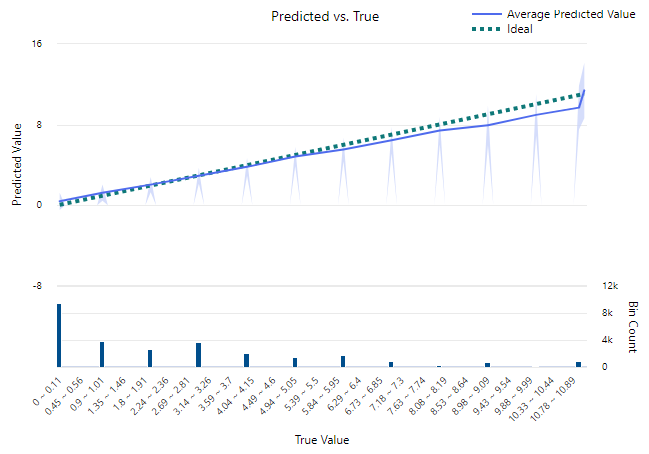
\includegraphics[width=0.48\textwidth]{figures/regression1Graph.png}
	\caption{The predicted values approximate the true values very well.}
	\label{fig:regression1Graph}
\end{figure}

However, Azure also provided insight into which attributes were most important to the accuracy of the model. As shown in Figure~\ref{fig:regression1ImportantFeatures}, the model relied heavily on class standing, term information, and demographic information. The distance to the front of the classroom falls in fifth place and attendance status in seventh.

\begin{figure}[ht]
  \centering
	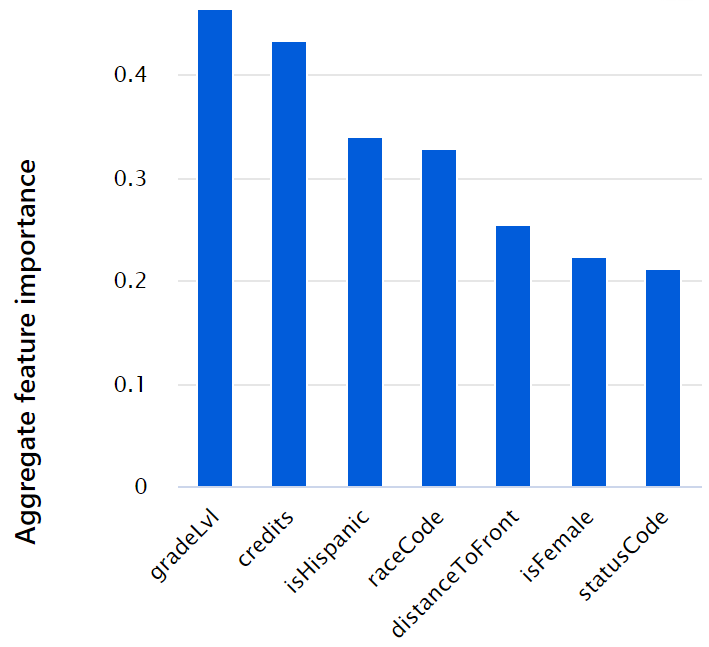
\includegraphics[width=0.48\textwidth]{figures/regression1ImportantFeatures.png}
	\caption{The top seven attributes used by the first regression model, ranked in order of predictive importance.}
	\label{fig:regression1ImportantFeatures}
\end{figure}

Based on the composition of other highly-accurate models, we suspect that the automated machine learning algorithm may have trained the regression model to recognize individual students and predict grades based on that student's historical performance.

To avoid this issue, the following experiment only retained two attributes, attendance status (statusCode) and distance to the front of the classroom (distanceToFront). After trying to correlate these attributes with the students' final grades for forty-eight minutes, the best model that Azure trained offered a mean absolute error that was nearly a fifth of the entire range. Very little of this error was explained by the variance in attendance data. Additionally, both correlation metrics suggested no correlation between the attendance data and student grades. In fact, the $R^2$ score suggests that there is a $95.7\%$ chance of getting this correlation from unrelated attributes.

\begin{table}[ht]
  \centering
  \caption{Regression Performance Metrics}
  \begin{tabular}[t]{lllll}
    \hline
    Attributes Used & RMSE & EV & Spearman & $R^2$ Score \\
    \hline
    All shown in SQL query & 1.110 & 0.859 & 0.906 & 0.859 \\
    statusCode, distanceToFront & 2.314 & 0.043 & 0.186 & 0.043 \\
    statusCode & 2.923 & 0.020 & 0.107 & 0.020 \\
    distanceToFront & 2.922 & 0.020 & 0.140 & 0.020 \\
    \hline
  \end{tabular}
  \label{tab:regressionMetrics}
\end{table}

Isolating the attendance status and seat row attributes even further did not improve results. Both prediction models produced separately by these two attributes yielded even lower correlation values.

Overall, the results of the correlation analysis showed that attendance and seat choice could not be used to accurately or precisely predict student grades in the data obtained from Southern Adventist University.

\subsection{Clustering}
Before other hyperparameters were tuned, the number of clusters, $k$, had to be decided. One approach, commonly called the ``Elbow Method,'' attempts to utilize the law of diminishing returns. As $k$ increases, the average size of each cluster naturally decreases. However, the number of clusters cannot be allowed to grow indefinitely. Thus, if several values for $k$ are tested and their average distance between a point and its assigned cluster is graphed, the inflection point can be selected as the best value for $k$. This method ensures that the average cluster size is relatively small while $k$ is also minimized.

\begin{figure}[ht]
  \centering
	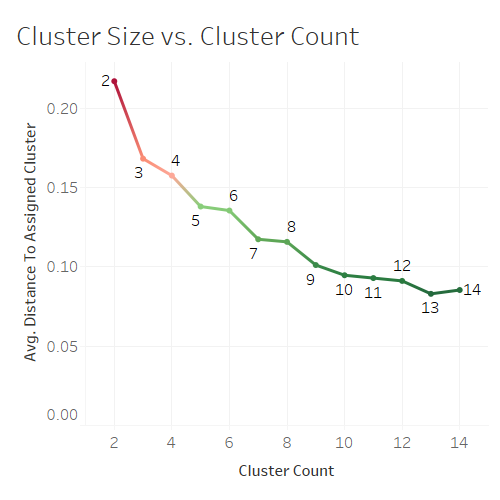
\includegraphics[width=0.48\textwidth]{figures/elbow.png}
	\caption{The average distance to a cluster compared across various number of clusters.}
	\label{fig:elbow}
\end{figure}

As shown in Figure~\ref{fig:elbow}, the inflection point is slightly unclear. Thus, experiments were first performed with $k=5$ clusters. The first experiment used all the queried columns. However, the clustering algorithm grouped data primarily using demographic information.\footnote{For example, four of the five clusters would be entirely based on a student's gender and hispanic status.}

After limiting the number of attributes available to the clustering algorithm, k-means grouped the data primarily based on attendance status and distance to the front of the classroom. However, five clusters proved too many for this set of attributes so the count was reduced to $k=3$.

The averages in Table~\ref{tab:3ClusterAvg} were obtained using three clusters and two input attributes. Data placed in Cluster 0 represented a mostly ``Present'' attendance status and a seat choice roughly halfway from the front of the classroom. Nearly all of the attendance records in this cluster had perfect scores of ``A''. Cluster 1 has similar averages, but with grades much closer to ``C+'' and ``C''. Finally, the cluster with chronically late attendance and a seating preference slightly beyond the halfway point has an average grade around a ``B+'' or ``B''.

\begin{table}[ht]
  \centering
  \caption{Average Attribute Values in Three Clusters}
  \begin{tabular}[t]{lllllll}
    \hline
    & status & distanceToFront & grade & 
    radius\tablefootnote{This feature was originally named ``Average Distance to Cluster Center'' and has been scaled so that the largest value is $1$.} & point count \\
    \hline
    Cluster 0 & 0.020 & 0.575 & 1.004 & 0.404 & 104833 \\
    Cluster 1 & 0.030 & 0.613 & 6.384 & 0.569 & 42212  \\
    Cluster 2 & 2.922 & 0.610 & 3.618 & 1.000 & 18143  \\
    Total     & 0.341 & 0.589 & 2.666 & 0.512 & 165188 \\
    \hline
  \end{tabular}
  \label{tab:3ClusterAvg}
\end{table}

The experiment was repeated with three clusters and no results wavered. Although Cluster 2 does show a group of students that is often late and performs worse than average, the three clusters together are inconclusive.

Finally, the experiments were repeated with only two clusters. The results are displayed in Table~\ref{tab:2ClusterAvg}. As seen before, distance to the front of the classroom is nearly the same for both clusters. However, Cluster 1 specifically represents records where a student was, on average, late to class. This cluster has an average grade between "B+" and "B". Cluster 0, on the other hand, displays much better attendance and grades on average between ``A-'' and ``B+''.

\begin{table}[ht]
  \centering
  \caption{Average Attribute Values in Two Clusters}
  \begin{tabular}[t]{lllllll}
    \hline
    & status & distanceToFront & grade & 
    radius\tablefootnote{See above.} & point count \\
    \hline
    Cluster 0 & 0.022 & 0.586 & 2.548 & 0.689 & 147033 \\
    Cluster 1 & 2.921 & 0.610 & 3.624 & 1.000 & 18155  \\
    Total     & 0.341 & 0.589 & 2.666 & 0.651 & 165188 \\
    \hline
  \end{tabular}
  \label{tab:2ClusterAvg}
\end{table}

Though interesting, these clusters are still far from ideal. One major issue is that they are unbalanced. One includes $89\%$ of the attendance data and the other only $11\%$. A more balanced dataset is desirable.

To further validate Azure's automated clustering algorithm, clustering was also performed in Weka 3.\footnote{\href{https://www.cs.waikato.ac.nz/ml/weka/}{cs.waikato.ac.nz/ml/weka}} The results from this experiment were identical to those obtained from Azure's k-means clustering.
